\section{Probes}

To observe a system, the outcomes, the result of causal links and outcome expressions, we must put probes in it.

For each outcome of interest, a probe (observation point) is attached to measure the delay of the outcome, like one would in a true oscilloscope. 

\iffalse
These probes allow to connect the system under test to the stub, which in turns sends outcome instances to the oscilloscope, which performs statistical computations on all the time series. 

Consider the figure below, a probe is attached at every component to measure the delay of N outcome ($p_2, p_3$), the stub will send the outcome instance data for each probe observing an outcome to the oscilloscope, which will measure their respective $\Delta$Qs from the time series data and display them (if chosen by the user). 
\fi

Consider the figure below, a probe is attached at every component to measure their $\Delta$Qs ($c_2, c_3$), 

Another probe ($p_1$) is inserted at the beginning and end of the system to measure the global execution delay. 

Thanks to this probe, the user can observe the $\Delta$Q \textit{"observed at $p_1$"}, which is the $\Delta$Q which was calculated from the data received by inserting probe $p_1$. The \textit{$\Delta$Q "calculated at $p_1$"} is the resulting $\Delta$Q from the convolution of the observed $\Delta$Qs at $c_2$ and $c_3$.   
    \begin{figure}[H]
        \begin{center}
            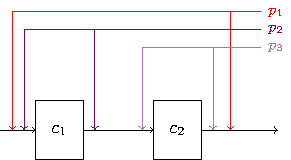
\includegraphics[scale=1.8]{tikz/probes.pdf}
        \end{center}
        \label{fig:probes}
        \caption{Probes inserted in a component diagram.}
    \end{figure}



